\documentclass[11pt, a4paper]{article}
\usepackage{polski}
\usepackage[utf8]{inputenc}
\usepackage[T1]{fontenc}
\usepackage[export]{adjustbox}
\usepackage{graphicx}
\usepackage{amsmath} 
\usepackage{listings}
\usepackage{color}
\usepackage{marvosym}
\usepackage{geometry}
\usepackage{enumerate}
\usepackage{float}
\usepackage{booktabs}
\usepackage{multirow}
\usepackage{titlesec}
\usepackage{hyperref}
\usepackage{tabularx}
\usepackage{amssymb}

\geometry{margin=1.2in}
\usepackage[final]{pdfpages}

\newcommand{\fbi}{\leavevmode{\parindent=1em\indent}}

\definecolor{dkgreen}{rgb}{0,0.6,0}
\definecolor{gray}{rgb}{0.5,0.5,0.5}
\definecolor{mauve}{rgb}{0.58,0,0.82}

\lstset{
	frame=tblr,
	language=Matlab,
	aboveskip=3mm,
	belowskip=3mm,
	showstringspaces=false,
	columns=flexible,
	basicstyle={\small\ttfamily},
	numbers=left,
	numberstyle=\tiny\color{gray},
	keywordstyle=\color{blue},
	commentstyle=\color{dkgreen},
	stringstyle=\color{mauve},
	breaklines=true,
	mathescape=false,
	breakatwhitespace=true,
	tabsize=3,
	inputencoding=utf8,
	extendedchars=true,
	literate=
	{ą}{{\k{a}}}1
	{Ą}{{\k{A}}}1
	{ę}{{\k{e}}}1
	{Ę}{{\k{E}}}1
	{ó}{{\'o}}1
	{Ó}{{\'O}}1
	{ś}{{\'s}}1
	{Ś}{{\'S}}1
	{ł}{{\l{}}}1
	{Ł}{{\L{}}}1
	{ż}{{\.z}}1
	{Ż}{{\.Z}}1
	{ź}{{\'z}}1
	{Ź}{{\'Z}}1
	{ć}{{\'c}}1
	{Ć}{{\'C}}1
	{ń}{{\'n}}1
	{Ń}{{\'N}}1
}

\renewcommand\lstlistingname{Listing}

\titleclass{\subsubsubsection}{straight}[\subsection]
\newcounter{subsubsubsection}[subsubsection]
\renewcommand\thesubsubsubsection{\thesubsubsection.\arabic{subsubsubsection}}
\renewcommand\theparagraph{\thesubsubsubsection.\arabic{paragraph}}

\titleformat{\subsubsubsection}
  {\normalfont\normalsize\bfseries}{\thesubsubsubsection}{1em}{}
\titlespacing*{\subsubsubsection}
{0pt}{3.25ex plus 1ex minus .2ex}{1.5ex plus .2ex}

\makeatletter
\renewcommand\paragraph{\@startsection{paragraph}{5}{\z@}
  {3.25ex \@plus1ex \@minus.2ex}
  {-0em}
  {\normalfont\normalsize\bfseries}}
\renewcommand\subparagraph{\@startsection{subparagraph}{6}{\parindent}
  {3.25ex \@plus1ex \@minus .2ex}
  {-1em}
  {\normalfont\normalsize\bfseries}}
\def\toclevel@subsubsubsection{4}
\def\toclevel@paragraph{5}
\def\toclevel@paragraph{6}
\def\l@subsubsubsection{\@dottedtocline{4}{7em}{4em}}
\def\l@paragraph{\@dottedtocline{5}{10em}{5em}}
\def\l@subparagraph{\@dottedtocline{6}{14em}{6em}}
\makeatother

\setcounter{secnumdepth}{4}
\setcounter{tocdepth}{4}

\hypersetup{pageanchor=false}

\setlength\parindent{3pt}

\renewcommand{\labelenumi}{\alph{enumi}.} 

\date{\today}


\begin{document}

\begin{titlepage}

\newcommand{\HRule}{\rule{\linewidth}{0.5mm}} 
\center 

\textsc{\LARGE Politechnika Wrocławska}\\[1.5cm] 
\textsc{\Large Inteligencja Obliczeniowa i jej zastosowania}\\[0.5cm] 
\HRule \\[0.5cm]
{ \huge \bfseries Ćwiczenie 1: Metody redukcji wymiarowości - analiza składowych głównych}\\[0.5cm] 
\HRule \\[1.6cm]
 
\begin{minipage}{0.4\textwidth}
\begin{flushleft} \large
\emph{Autorzy:}\\
Paweł  \textsc{Andziul} 200648 \\
Robert  \textsc{Chojnacki} 200685 \\
Marcin  \textsc{Słowiński} 200638 \\
\end{flushleft}
\end{minipage}
~
\begin{minipage}{0.4\textwidth}
\begin{flushright} \large
\emph{Prowadzący:} \\
dr hab. inż. Rafał \textsc{Zdunek}
\end{flushright}
\end{minipage}\\[4cm]

\vfill 
{\large 31 maja 2017}\\[3cm] 

\end{titlepage}

\tableofcontents

\newpage

\section{Zadanie 1}
\paragraph{}
Dla danych:
\begin{center}
\(X = [2.5 0.5 2.2 1.9 3.1 2.3 2 1 1.5 1.1; 2.4 0.7 2.9 2.2 3 2.7 1.6 1.1 1.6 0.9];\)
\end{center}
\begin{enumerate}[a.]
	\item Zaimplementować metodę PCA w Matlabie. Do wyznaczenia par własnych macierzy kowariancji można zastosować wbudowaną funkcję eig(.) lub eigs(.).
	\item Wyznaczyć składowe główne i wektory cech.
	\item Pokazać na rysunku punkty obserwacji oraz wyznaczone wielkości.
\end{enumerate}

\subsection{Opis metody}
\paragraph{}
Metoda PCA (ang. \textit{Principal Component Analysis}) jest jedną ze statystycznych metod analizy czynnikowej, która pozwala na odnajdywanie pewnych struktur w zbiorze zmiennych losowych. Analiza składowych głównych oparta jest na wykorzystaniu pojęć ze statystyki, jakimi są m.in. korelacja i wariancja. Wielowymiarowe dane z reguły nie są równomiernie rozrzucone wzdłuż wszystkich kierunków układu współrzędnych, ale koncentrują się w pewnych podprzestrzeniach oryginalnej przestrzeni. Celem PCA jest znalezienie tych podprzestrzeni w postaci składowych głównych, tzn. kierunków przy których wartość wariancji (lub korelacji) jest zmaksymalizowana. Analiza może być oparta albo na macierzy korelacji, albo macierzy kowariancji utworzonych ze zbioru wejściowego.

\fbi
Metoda PCA jest zazwyczaj używana do redukcji rozmiaru danych poprzez odrzucenie ostatnich czynników, tzn. takich, których wariancja jest najniższa. Oznacza to, że \textit{n}-wymiarowy zbiór danych możemy ograniczyć wyznaczając \textit{n}-wektorów własnych, z których wybieramy tylko \textit{k}-wektorów, tak aby $k \le n$. Zrzutowanie danych na przestrzeń rozpiętą przez \textit{k}-wybranych wektorów pozwala zredukować wymiarowość danych.

\subsection{Algorytm}
\paragraph{}
Jako dane wejściowe podawana jest macierz zawierająca kolejne obserwacje, na podstawie których będą wyznaczane główne składowe. Algorytm PCA składa się z następujących kroków:
\begin{enumerate}[1.]
	\item Wyznaczenie wartości średnich dla wierszy 
	\item Odjęcie od macierzy wejściowej wyliczonych poprzednio średnich
	\item Wyznaczenie macierzy kowariancji
	\item Wyznaczenie składowych głównych
	\item Wybór najlepszych składowych
	\item Rzutowanie na wektory własne
\end{enumerate}

\fbi
Na początku należy przeprowadzić normalizację. W ten sposób zapewniamy, że cechy szerzej rozłożone nie zdominują cech mocniej skoncentrowanych. Normalizacja polega na wyznaczeniu średnich wartości kolejnych cech dla wszystkich obserwacji. Następnie od macierzy wejściowej odejmujemy wcześniej wyliczone średnie - od każdego elementu macierzy odejmujemy średnią dla wiersza, w którym się znajduje. Dla tak uzyskanych danych należy policzyć macierz kowariancji.

\fbi
Kolejnym krokiem jest wyznaczenie wektorów i wartości własnych. Wylicza się \textit{k}-ortonormalnych wektorów, które tworzą bazę dla unormowanych danych wejściowych. Są to wektory jednostkowe, wskazujące w kierunku prostopadłym do pozostałych wektorów z utworzonej bazy. Liczba wektorów własnych jest związana z wymiarem rozpatrywanych danych, a wartości własne określają długość wektora.

\fbi
Następnie porządkujemy wartości własne w kolejności malejącej. Redukcja opiera się na wyborze wektorów własnych z największą wartością własną. Można powiedzieć, że maksymalizujemy zmienność danych wraz z jednoczesną minimalizacją ubytku informacji spowodowanej ich redukcją. Redukcja dokonuje się poprzez mnożenie macierzy wybranych wektorów przez \textit{n}-wymiarową macierz danych.

\fbi
Jeżeli wybierzemy mniejszą liczbę wektorów własnych (\textit{k} z \textit{n}) otrzymujemy zredukowaną przestrzeń danych. Prowadzi to do utraty części oryginalnej informacji, a rozmiar straty zależy od doboru wektorów. Jeżeli wybierzemy wszystkie wektory własne, uzyskujemy jedynie obrót macierzy danych wejściowych, bez utraty żadnych informacji.

\subsection{Realizacja}
\paragraph{}
Opracowano skrypt w środowisku Matlab realizujący metodę PCA zgodnie z algorytmem opisanym wcześniej. Wykorzystano wbudowane funkcję do obliczenia i odjęcia wartości średnich (mean(.), bsxfun(.)) oraz do wyznaczenia macierzy kowariancji (cov(.)). W celu obliczenia par własnych macierzy kowariancji zastosowana została metoda eigs(.), w której pierwszym argumentem jest macierz kowariancji, a drugim ilość wektorów własnych.

\lstinputlisting[label=lst:zad1,caption=Wyznaczanie wartości własnych i wektorów własnych,firstline=1,lastline=50]{./assets/skrypt_zad1.m}

\fbi
Pozostałe funkcje służą do wykreślenia wykresu zawierającego kolejno: dane wejściowe, składowe główne oraz wyznaczone wektory własne. 

\subsection{Wyniki}
\paragraph{}
Dane wejściowe, składowe główne oraz wektory własne przedstawiono na rysunku \ref{fig:zad1}. Wyznaczone wektory i wartości własne przedstawiono w tabelach \ref{tab:wektory-wlasne} oraz \ref{tab:wartosci-wlasne}. Można zauważyć, że zgodnie z założeniami metody PCA, wektory własne są ortogonalne. Jeden z wektorów pokazuje kierunek, w którym wariancja jest największa.

\begin{figure}[H]
	\centering
	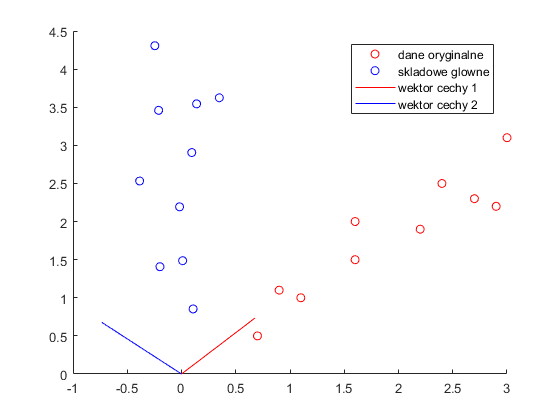
\includegraphics[width=0.95\textwidth]{./assets/ilustracja_zad1_normalizacja.png}
	\caption{Ilustracja punktów obserwacji i składowych głównych}
	\label{fig:zad1}
\end{figure}

\begin{table}[H]
	\centering
	\caption{Wyznaczone wektory własne.}
	\begin{tabular}{c|c|c|}
		\cline{2-3}
		& x & y \\ 
		\hline
		\multicolumn{1}{|c|}{wektor cechy 1} & 0.7352 & 0.6779 \\ 
		\hline 
		\multicolumn{1}{|c|}{wektor cechy 2} & 0.6779 & -0.7352 \\
		\hline 
	\end{tabular}
	\label{tab:wektory-wlasne}
\end{table}


\begin{table}[H]
	\centering
	\caption{Wyznaczone wartości własne.}
	\begin{tabular}{|c|c|}
		\hline 
		wektor cechy 1 & 1.2840 \\ 
		\hline 
		wektor cechy 2 & 0.0491 \\ 
		\hline
	\end{tabular}
	\label{tab:wartosci-wlasne}
\end{table}

\fbi
Na wykresie można zauważyć poprawne działanie funkcji PCA. Dane rozkładają się wzdłuż oznaczonych wektorów.

\section{Zadanie 2}
\paragraph{}
Dla obrazów twarzy z bazy ORL (lub podobnej) wyznaczyć cechy holistyczne (twarze własne) dla różnej liczby estymowanych komponentów głównych (\(J = 4, 10, 20, 30\)). Pogrupować obrazy stosując metodę \textit{k}-średnich, do obrazów oryginalnych oraz redukowanych. Badania przeprowadzić dla różnej liczby grup. Porównać dokładność i czas grupowania. Następnie dokonać klasyfikacji obrazów w obu przestrzeniach (oryginalnej i zredukowanej) za pomocą klasyfikatora \textit{k-NN}. Porównać efekty klasyfikacji z efektami grupowania.

\subsection{Wczytanie obrazów twarzy}
\paragraph{}
Na ilustracji \ref{fig:ilustracja_zad2_dane} zamieszczono wykorzystane dane twarzy 3 różnych osób. Oryginalne twarze pochodzą ze strony \cite{test6}. Zdjęcia twarzy są już znormalizowane.

\begin{figure}[H]
	\centering
	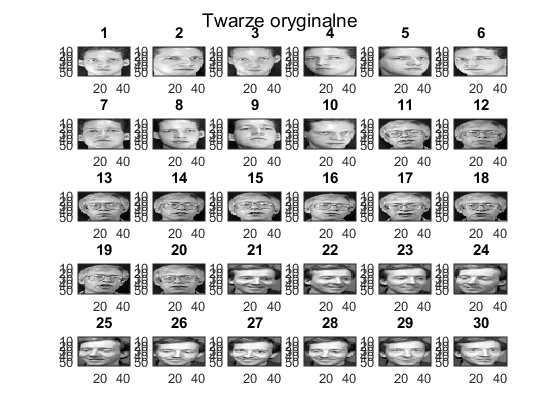
\includegraphics[width=0.95\textwidth]{./assets/ilustracja_zad2_dane.png}
	\caption{Obrazy twarzy wykorzystane do obliczeń}
	\label{fig:ilustracja_zad2_dane}
\end{figure}

\lstinputlisting[label=lst:zad2b,caption=Wczytywanie danych twarzy do macierzy,firstline=1,lastline=25]{./assets/skrypt_zad2.m}

\subsection{Wyznaczenie cech holistycznych (twarzy własnych)}
\paragraph{}
Do wyznaczania twarzy własnych zastosowano podobnie jak w zadaniu poprzednim metodę PCA. Na listingu \ref{lst:zad2b} fragment odpowiedzialny za ten etap.

\lstinputlisting[label=lst:zad2b,caption=Wyznaczanie twarzy własnych,firstline=25,lastline=40]{./assets/skrypt_zad2.m}

\begin{figure}[H]
	\centering
	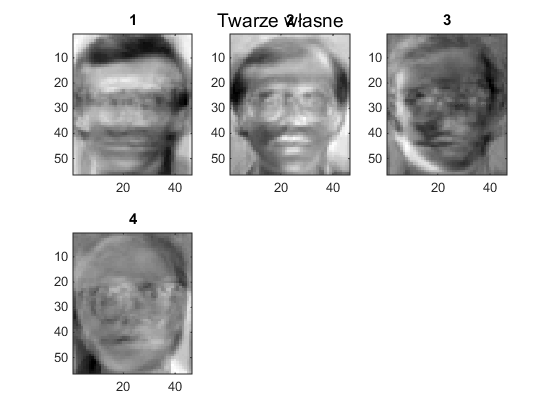
\includegraphics[width=0.95\textwidth]{./assets/ilustracja_zad2_eigen_j4.png}
	\caption{Wyznaczone twarze własne J=4}
	\label{fig:ilustracja_zad2_eigen_j4}
\end{figure}

\begin{figure}[H]
	\centering
	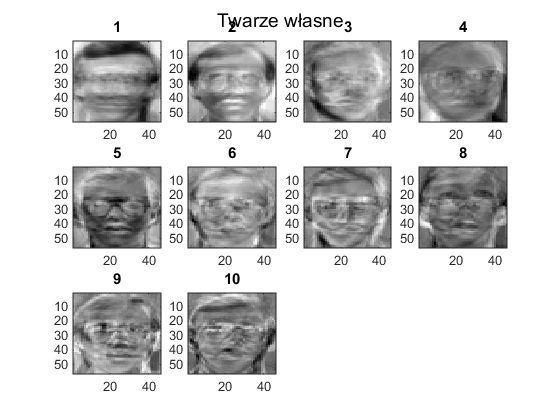
\includegraphics[width=0.95\textwidth]{./assets/ilustracja_zad2_eigen_j10.png}
	\caption{Wyznaczone twarze własne J=10}
	\label{fig:ilustracja_zad2_eigen_j10}
\end{figure}

\begin{figure}[H]
	\centering
	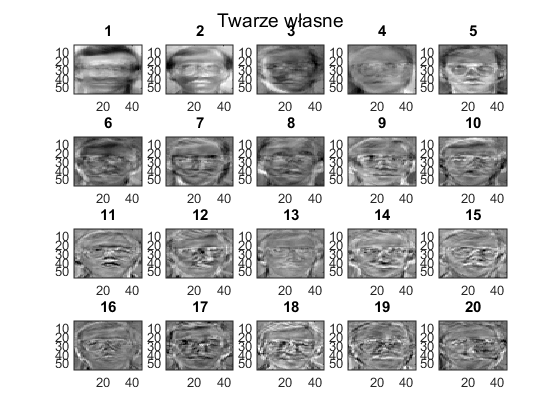
\includegraphics[width=0.95\textwidth]{./assets/ilustracja_zad2_eigen_j20.png}
	\caption{Wyznaczone twarze własne J=20}
	\label{fig:ilustracja_zad2_eigen_j20}
\end{figure}

\begin{figure}[H]
	\centering
	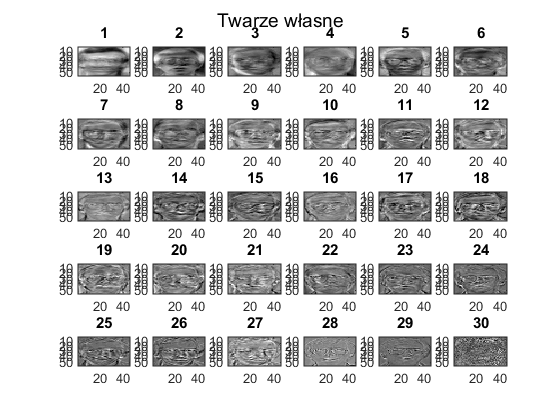
\includegraphics[width=0.95\textwidth]{./assets/ilustracja_zad2_eigen_j30.png}
	\caption{Wyznaczone twarze własne J=30}
	\label{fig:ilustracja_zad2_eigen_j30}
\end{figure}

\subsection{Grupowanie metodą k-średnich}
\paragraph{}


\lstinputlisting[label=lst:zad2c,caption=Grupowanie twarzy oryginalnych i własnych ,firstline=63,lastline=80]{./assets/skrypt_zad2.m}

Wyniki grupowania dla obrazów oryginalnych dla różnych rozmiarów grup przedstawiono w tabeli \ref{tab:wynikiGrupowaniaZwykle}.

\begin{table}[H]
	\centering
	\caption{Jakość grupowania dla różnych wielkości grup (n) dla obrazów oryginalnych}
	\begin{tabular}{|c|c|c|}
		\hline 
		n & AccMeasure & Czas przetwarzania [s] \\ 
		\hline
		1 & 33.33 & 0.886 \\
		\hline
		2 & 66.67 & 0.168 \\
		\hline
		3 & 100.00 & 0.113 \\
		\hline
	\end{tabular}
	\label{tab:wynikiGrupowaniaZwykle}
\end{table}

Wyniki grupowania dla twarzy własnych dla różnych wartości J przedstawiono w tabeli \ref{tab:wynikiGrupowaniaWlasne}.

\begin{table}[H]
	\centering
	\caption{Jakość grupowania dla różnych wartości J dla twarzy własnych}
	\begin{tabular}{|c|c|c|}
		\hline 
		J & AccMeasure & Czas przetwarzania [s] \\ 
		\hline
		3 & 50.00 & 0.057 \\
		\hline
		10 & 50.00 & 0.048 \\
		\hline
		20 & 65.00 & 0.062 \\
		\hline
		30 & 80.00 & 0.020 \\
		\hline
	\end{tabular}
	\label{tab:wynikiGrupowaniaWlasne}
\end{table}

\subsection{Klasyfikacja za pomocą klasyfikatora k-NN}
\paragraph{}
Zgodnie z dokumentacją metody knnclassify \cite{test3} umożliwia ona klasyfikację pewnej próbki danych na podstawie danych dla których klasyfikacja jest znana.

\begin{equation}\label{eq:knnclasify}
Class = knnclassify(Sample, Training, Group)
\end{equation}

, parametry $Training$ oraz $Group$ zawierają informację o podziale danych na grupy natomiast $Sample$ jest zbiorem którego klasyfikację pragniemy przeprowadzić. Wynikiem jest $Class$ będący tego samego typu co $Group$ tzn. dziedzina klasyfikacji jest taka sama.

Poniżej (listing \ref{lst:zad2d}) zamieszczono implementację klasyfikacji.

\lstinputlisting[label=lst:zad2,caption=Fragment skryptu w Matlabie obejmujący klasyfikację k-NN,firstline=80,lastline=100]{./assets/skrypt_zad2.m}



\begin{figure}[H]
	\centering
	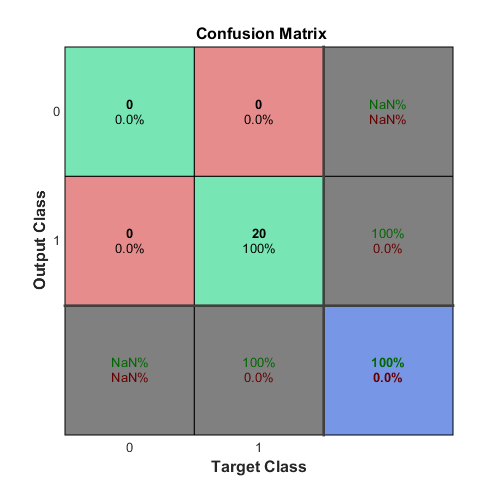
\includegraphics[width=0.75\textwidth]{./assets/ilustracja_zad2_conf_j20.png}
	\caption{Confusion matrix dla J=20}
	\label{fig:ilustracja_zad2_conf_j20}
\end{figure}



\section{Zadanie 3}
\paragraph{}
Wyznaczyć pary własne macierzy kowariancji za pomocą algorytmów: Powera oraz Lanczosa. Zaimplementować algorytmy i zastosować je do rozwiązania powyższych zadań. Porównać wyniki.

\subsection{Algorytm Powera}
\paragraph{}

\lstinputlisting[label=lst:zad3,caption=Fragment skryptu w Matlabie,firstline=1,lastline=500]{./assets/Power_f.m}

\fbi
Algorytm Powera polega na kolejnym przemnażaniu macierzy wejściowej przez wektor wynikowy do momentu, gdy wektor uzyskany w wyniku działania nie różni się bardziej od wynikowego o więcej niż założona wartość tolerancji.

\fbi
Powyższe założenie wynika z faktu, że kolejne wektory dążą do pewnej zwielokrotnionej wartości. Ważnym jest by tę wartość wychwycić nie wykonując nadmiarowych obliczeń.

\fbi
W zaimplementowanej funkcji przechowywane są dwa wektory - stary i nowy. Wektory te odejmowane są od siebie i normalizowane. Jeżeli różnica między nimi jest mniejsza niż założona tolerancja zwracany jest wektor nowszy jako bliższy idealnemu rozwiązaniu.

\subsection{Algorytm Lanczosa}
\paragraph{}

\subsection{Wyniki}
\paragraph{}

\section{Podsumowanie}
\paragraph{}
Podczas zajęć laboratoryjnych zapoznano się z metodą PCA. Poznano również podstawy grupowania i klasyfikacji danych z wykorzystaniem pakietu Matlab.


\newpage
\begin{thebibliography}{40}

\bibitem{test1}
\url{https://www.mathworks.com/help/nnet/ref/plotconfusion.html}

\bibitem{test2}
\url{https://www.mathworks.com/help/stats/confusionmat.html}

\bibitem{test3}
\url{https://www.mathworks.com/help/bioinfo/ref/knnclassify.html}

\bibitem{test4}
\url{http://www.kmg.zut.edu.pl/opt/wyklad/bezgrad/powell.html}

\bibitem{test5}
\url{https://en.wikipedia.org/wiki/Lanczos_algorithm}

\bibitem{test6}
\url{http://www.cl.cam.ac.uk/research/dtg/attarchive/facedatabase.html}

\bibitem{test7}
Berk Gokberk, ,,Assignment 2: Face Recognition using PCA'',
\url{http://www2.cmpe.boun.edu.tr/courses/cmpe58Z/spring2010/files/assignment2_new.pdf}


\end{thebibliography}

\end{document}
